\documentclass[journal,final]{new-aiaa}
\usepackage[utf8]{inputenc}
\usepackage{color}
\usepackage{algorithm}
\usepackage[noend]{algpseudocode}
\usepackage{graphicx}
\usepackage{amsmath}
\usepackage[version=4]{mhchem}
\usepackage{siunitx}
\usepackage{longtable,tabularx}
\setlength\LTleft{0pt}

\newcommand{\A}{\mathbf{A}}
\newcommand{\B}{\mathbf{B}}
\newcommand{\C}{\mathbf{C}}
\newcommand{\D}{\mathbf{D}}
\newcommand{\E}{\mathbf{E}}
\newcommand{\F}{\mathbf{F}}
\newcommand{\G}{\mathbf{G}}
\newcommand{\HH}{\mathbf{H}}
\newcommand{\I}{\mathbf{I}}
\newcommand{\J}{\mathbf{J}}
\newcommand{\K}{\mathbf{K}}
\newcommand{\LL}{\mathbf{L}}
\newcommand{\PP}{\mathbf{P}}
\newcommand{\R}{\mathbf{R}}
\newcommand{\U}{\mathbf{U}}
\newcommand{\W}{\mathbf{W}}
\newcommand{\w}{\mathbf{w}}

\newcommand{\uu}{\mathbf{u}}
\newcommand{\n}{\mathbf{n}}
\newcommand{\rr}{\mathbf{r}}
\newcommand{\s}{\mathbf{s}}
\newcommand{\e}{\mathbf{e}}
\newcommand{\ddd}{\mathbf{d}}
\newcommand{\f}{\mathbf{f}}
\newcommand{\T}{\mathbf{T}}
\newcommand{\x}{\mathbf{x}}
\newcommand{\y}{\mathbf{y}}
\newcommand{\ttt}{\mathbf{t}}
\newcommand{\bb}{\mathbf{b}}

\newcommand{\vv}{\mathbf{v}}
\newcommand{\boldalpha}{\boldsymbol{\alpha}}


\newcommand{\df}[2]{\dfrac{\partial#1}{\partial#2}}
%\newcommand{\dd}[3]{\dfrac{\partial^2#1}{\partial#2 \partial#3}}
\newcommand{\dd}[3]{{\partial^2#1}/{\partial#2 \partial#3}}
\newcommand{\ff}[2]{\dfrac{d#1}{d#2}}
\newcommand{\ds}[2]{\dfrac{\partial^2#1}{\partial#2^2}}
\newcommand{\dn}[3]{\dfrac{\partial^{#1}#2}{\partial#2^{#1}}}

\newcommand{\dis}{\displaystyle}

\newcommand{\npo}{n\!\!+\!\!1}

\newcommand{\grad}{\textrm{grad\,}}
\newcommand{\Div}{\textrm{div\,}}

\newcommand{\half}{\frac{1}{2}}
\newcommand{\third}{\frac{1}{3}}
\newcommand{\quarter}{\frac{1}{4}}

\newcommand{\Atv}{\A^{\!T}\!v}
\newcommand{\Au}{\A u}
\newcommand{\RK}{R-K\@\xspace}
\newcommand{\vtf}{v^T\!f}
\newcommand{\gtu}{g^T\!u}

\newcommand{\degr}{^{\circ}}
\newcommand{\logt}{\log_{10}}
\newcommand{\dsps}{\displaystyle\strut}

\newcommand{\ind}{\phantom{\bf do}}

\graphicspath{{./pic/}}

\title{Flow instability inception prediction using eigenvalue analysis}
\author[1]{Shenren Xu	
\footnote{ Email address: shenren\_xu@nwpu.edu.cn}}
\affil[1]{School of Power and Energy, 
	Northwestern Polytechnical University, Xi'an, 710072, China}
\author[1]{Zhihao Wu
}


\begin{document}
\maketitle

\begin{abstract}
The compression system in turbomachines, e.g.,  aircraft engines and gas turbines,
when operating under off-design conditions, exhibits flow instability such as surge, rotating stallm leading to performance deterioration, noises and structural damages.
Inability to accurately predict the condition under which such flow instability will
happen severe hinders the development of high performance compression system.
In this work,  an eigenvalue analysis method is developed to predict flow stability
commonly seen for turbomachines operating at near stall conditions. The eigenvalue
analysis is fully based on the steady state three-dimensional Reynods-averaged
Navier-Stokes equations and thus the stability boundary is fully consistent with
the one that is predicted by the time-accurate flow simulation, i.e., URANS, but
two to three times faster.
The method is applied to the computation of stability boundary of
(i) the laminar flow around a two-dimensional circular cylinder,
(ii) the flow around a quasi-three-dimensional compressor anuular cascade, 
and 
(iii) flow around a three-dimensional compressor rotor.
The method developed here has the potential to revive
the once-popular eigenvalue method for prediction rotating stall and surge, which
was based on lower-fidelity flow models and provide industry with tools to
accurately predict the stall line in the early design stage.
\end{abstract}

%\section*{Nomenclature}
%{\renewcommand\arraystretch{1.0}
%\noindent\begin{longtable*}{@{}l @{\quad=\quad} l@{}}
%$c_v,c_p$   & specific heat \\
%$e$     & internal energy\\
%$E$     & total energy\\
%
%$\partial \Omega_r$& boundary of $\Omega_r$
%\end{longtable*}}

\section{The nonlinear flow solver}
%The nonlinear flow solver used in this work is NutsCFD, an unstructured
%finite volume Reynolds-averaged Navier--Stokes solver capable of dealing
%with rotating frame reference and periodic boundary conditions.
%The solver features the use of a noval Newton--Krylov algorithm,
%which significantly enhances the efficiency and robsutness when
%computing turbomachinery flows at off-design conditions.
%Details of the NK algorithm can be found in~\cite{123} and
%only general information of the solver theory is provided below.

\subsection{Governing equations}
%The integral form of the governing equations in a
%relative frame of reference with an angular
%velocity of $\boldsymbol \omega$ is
%\begin{equation*}
%\dfrac{d}{dt}\int_{\Omega_r} \W dV
%+\oint_{\partial \Omega_r} (\F^r_c-\F_v)dS
%+\int_{\Omega_r}\F_\omega dS
%=0,
%\label{governing}
%\end{equation*}
%where $\W$ are %is
%the conservative variables
%$\left[\rho,~\rho\uu,~\rho E\right]^T$.
%The absolute and relative convective fluxes,
%$\F_c$ and $\F^r_c$,
%the viscous flux $\F_v$,
%and the additional flux due
%to rotation, $\F_\omega$,
%are defined as %follows
%\begin{equation*}
%\F_c=
%\left [ 
%\begin{array}{c}
%\rho \uu \cdot \n\\
%\rho \uu \uu\cdot \n +  p\n\\
%\rho H \uu \cdot \n
%\end{array}
%\right],
%\text{~~}
%\F^r_c=
%%\left [ 
%%\begin{array}{c}
%%\rho \uu \cdot \n\\
%%\rho \uu \uu\cdot \n +  p\n\\
%%\rho H \uu \cdot \n
%%\end{array}
%%\right]
%\F_c
%-
%(\uu_{rot}\cdot \n) 
%\left [ 
%\begin{array}{c}
%\rho\\
%\rho \uu\\
%\rho E
%\end{array}
%\right ]
%,\text{~~}
%\F_v=
%\left [ 
%\begin{array}{c}
%0\\
%\tau \cdot \n\\
%\uu \cdot \tau \cdot \n + \kappa \n \cdot \nabla T
%\end{array}
%\right ],\text{~~}
%\F_\omega=
%\left [ 
%\begin{array}{c}
%0\\
%\rho {\boldsymbol{\omega}} \times \uu\\
%0
%\end{array}
%\right ],
%\end{equation*}
%with $\uu_{rot}={\boldsymbol \omega} \times \x$.


\subsection{Spatial discretization}
%The governing equations are discretized using the
%method of lines and thus the spatial and temporal
%discretizations can be treated separately.
%The governing equations for the
%steady state solution $\W$ is
%\begin{equation}
%\R(\W)={\bf 0},
%\label{nonlinear}
%\end{equation}
%where $\R$ is the sum of fluxes and source terms
%associated with each control volume. Suppose control
%volume %node
%$i$ has $N$ flux faces with
%area $S_{ik}$ for
%$k=1,2,...,N$.
%$R_i$ then is 
%\begin{equation*}
%R_i(\W)=\sum^{N}_{k=1} (\F^r_c-\F_v)S_{ik}+\F_{\omega} V_i,
%\end{equation*}
%where $V_i$ denotes the volume.
%
%Turbulence is modelled using the negative Spalart--Allmaras
%(SA-neg) model~\cite{allmaras2012modifications}.
%Compared to the original SA model~\cite{allmaras2012modifications},
%this avoids the clipping of the turbulent variable
%to a non-negative value which potentially
%prevents the full convergence of the nonlinear solver.
%The turbulence equation is discretized using
%the first-order accurate upwind
%scheme~\cite{langer2014agglomeration}.
%
%\subsection{Temporal discretization}
%The time-marching of the nonlinear equation is
%based on Newton's method.
%Equation~\eqref{nonlinear} is solved by iteratively updating
%the solution as
%\begin{equation*}
%  \W^{n+1}=\W^n+ \Delta \W
%  \label{newtonTransient}
%\end{equation*}
%until convergence is reached, i.e., $\|\R(\W)\|=0$,
%where $\Delta \W$ is the solution to the linear 
%system of equations
%\begin{equation*}
%  \df{\R}{\W}\Delta \W = -\R(\W^n) 
%\end{equation*}
%The exact Jacobian matrix is computed with the
%help of automatic differentiation tool
%Tapenade~\cite{Tapenade}
%and the graph coloring package
%Colpack~\cite{gebremedhin2013colpack}.
%The sparse linear system of equations arising
%from the linearization of $\R$ is solved with
%the Krylov-subspace solver, GMRES, with
%incomplete LU factorization (ILU) as the
%preconditioner. The overall algorithm
%is the Newton--Krylov (NK) method. Special care is
%taken to handle the periodic boundary condition
%when simulating flows in a single passage.

\section{Stability analysis}
\subsection{Time-domain unsteady approach}
\subsection{Eigenvalue approach}
\section{Eigenvalue analysis for large sparse matrices}

\section{Results}
\label{results}

\subsection{Laminar flow around a two-dimensional circular cylinder}

\subsubsection{Steady state calculation}
\subsubsection{Unsteady calculation}
\subsubsection{Eigenvalue analysis}

%
%We use the NutsCFD to compute the steady state laminar flow around the
%circular cylinder for Reynolds number 50, 60 and 75. Eigenvalue analysis is
%performed for each case. The three spectra is shown in Fig.~\ref{fig:cyl}.
%It can be seen that linearly unstable mode start to appear from Re=60.
%The unstable mode at Re=60 is visualized on the right in Fig.~\ref{fig:cyl}
%where our results based on the NutsCFD solver is compared to that
%computed using Nektar++~\cite{cantwell2015nektar++}.
%
%\begin{figure}[htb]
%	\centering   
%	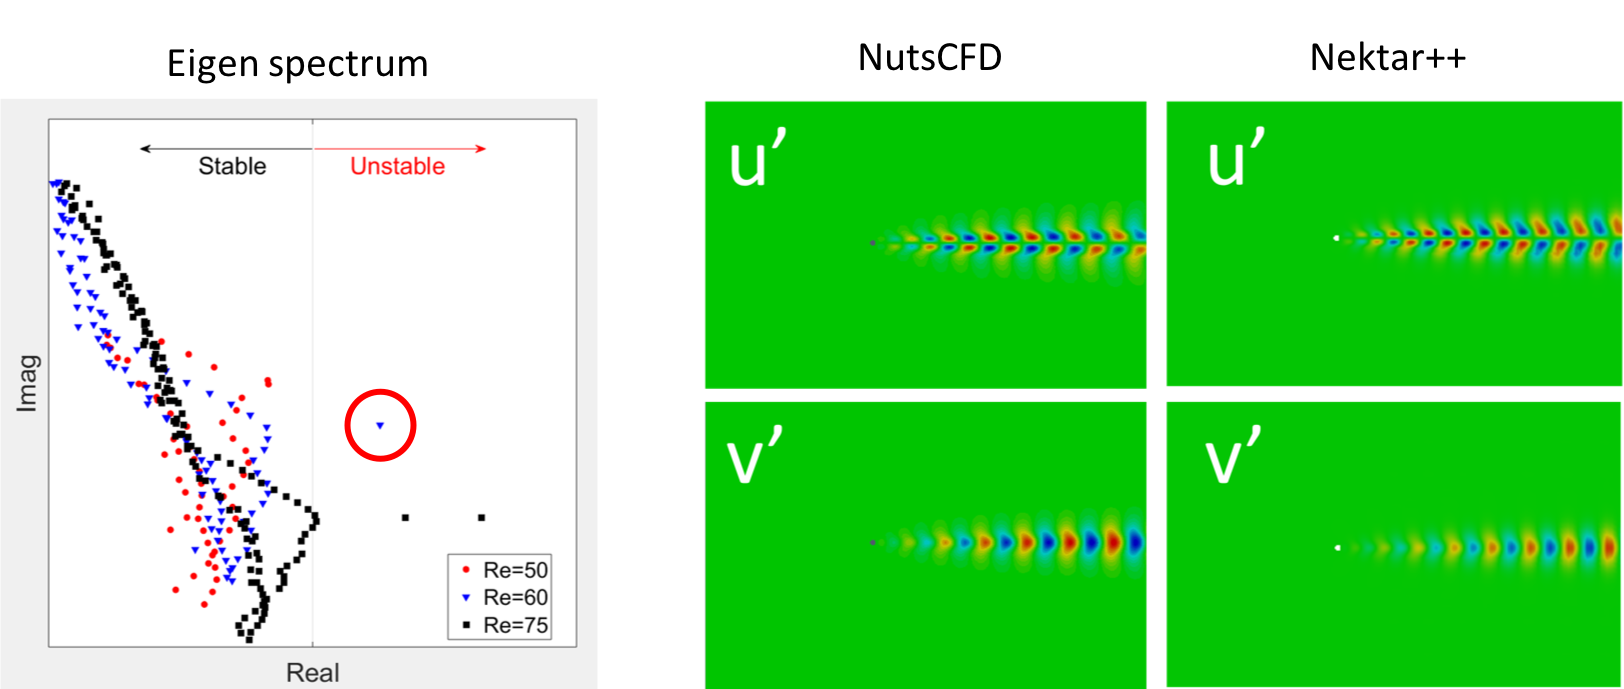
\includegraphics[width=0.99\textwidth]{pic/cyl.png}
%	\caption{Left: spectra computed for the laminar flow around circular cylinder
%		at different Reynolds number; right: x- and y-velocity components
%		of the unstable eigenvector computed by NutsCFD compapred with
%		that with Nektar++.}
%	\label{fig:cyl}
%\end{figure}

\subsection{Rotating stall for an annular compressor cascade}

\subsubsection{Steady state calculation}
\subsubsection{Unsteady calculation}
\subsubsection{Eigenvalue analysis}

\subsection{Rotating instability for an axial compressor rotor}

\subsubsection{Steady state calculation}
\subsubsection{Unsteady calculation}
\subsubsection{Eigenvalue analysis}

\section{Conclusion}
\label{conclusion}

\section*{Acknowledgements}

\bibliography{xu}

\end{document}
